\textbf{See the instruction for questions \inteval{\value{question}+1} to \inteval{\value{question}+3}.}

General instruction (if any) goes here.

\begin{center}
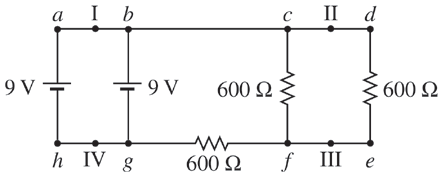
\includegraphics[scale=0.5]{images/img-006-017.png}
\end{center}

Two $9\unit{V}$ batteries and three identical $600\latinunit{\Omega}$ resistors are connected in a circuit, as shown above. Neglect internal resistance in the batteries and consider all meters to be ideal.

% Multiple Choice Question 19
\begin{questions}\setcounter{question}{18}\question
A voltmeter would read $6\unit{V}$ if connected correctly between which two points in the circuit?

\begin{oneparchoices}
\choice $a$ and $b$
\choice $a$ and $f$
\choice $b$ and $f$
\choice $c$ and $d$
\choice $f$ and $g$
\end{oneparchoices}\end{questions}

% Multiple Choice Question 20
\begin{questions}\setcounter{question}{19}\question
Ammeters are inserted at points I, II, III, and IV. At which of the other points would the ammeter register the same current as the ammeter at point IV ?

\begin{oneparchoices}
\choice I only
\choice III only
\choice I and II only
\choice II and III only
\choice I, II, and III
\end{oneparchoices}\end{questions}

% Multiple Choice Question 21
\begin{questions}\setcounter{question}{20}\question
What is the total power dissipated in the three resistors?

\begin{oneparchoices}
\choice $0.023 \unit{W}$
\choice $0.045 \unit{W}$
\choice $0.090 \unit{W}$
\choice $0.36 \unit{W}$
\choice $9.0 \unit{W}$
\end{oneparchoices}\end{questions}

